\section{Introduction}

\begin{frame}<1>[fragile,label=f1]
    \frametitle<1>{The power of parallel workers}
    \frametitle<2>{P2P comms: A first example}
    \frametitle<3>{Oh, there is a reduce here!}
    \frametitle<4>{What if one of them just walks away mid-op?}
    \begin{figure}
        \begin{center}
        \begin{tikzpicture}
            \node[anchor=south west,inner sep=0] at (0,0) {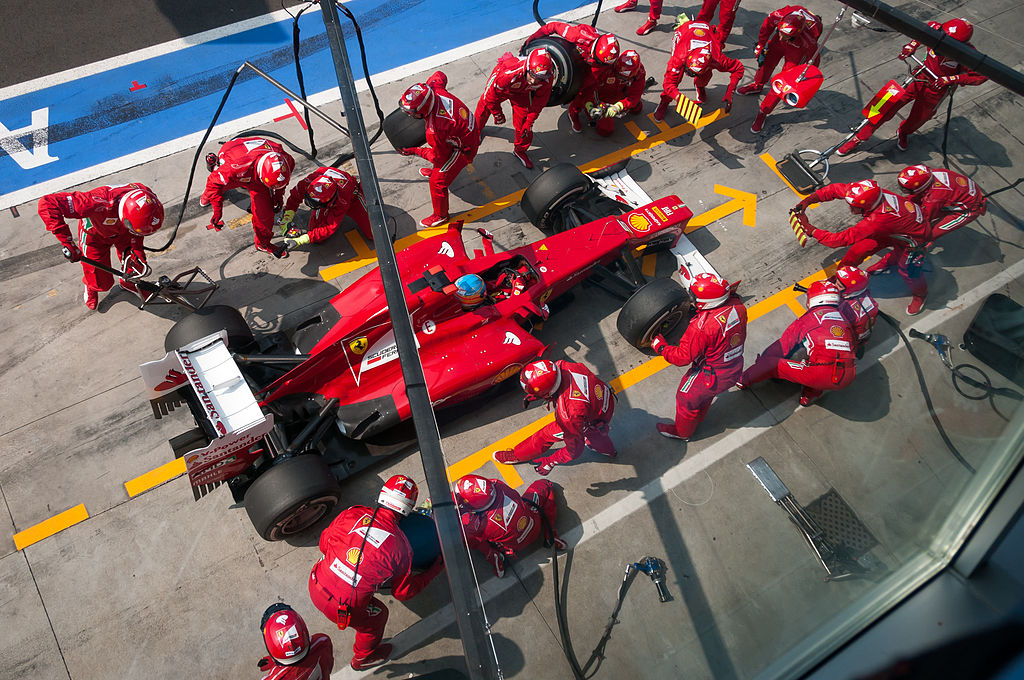
\includegraphics[height=0.7\pageheight]{images/Ferrari_pit_stop.jpg}};
            \draw<2>[mLightGreen,ultra thick,fill=mLightGreen,fill opacity=.2] (4.5,5) rectangle (6,6);
            \draw<2>[mLightGreen,ultra thick,fill=mLightGreen,fill opacity=.2] (5,3.5) rectangle (6.5,4.5);

            \draw<3>[mLightBrown,ultra thick,fill=mLightBrown,fill opacity=.2] (7,5) rectangle (8,6);
            \draw<3>[mLightGreen,ultra thick,fill=mLightGreen,fill opacity=.2] (4,3) rectangle (5,4);
            \draw<3>[mLightGreen,ultra thick,fill=mLightGreen,fill opacity=.2] (7,3.5) rectangle (8,4.5);
            \draw<3>[mLightGreen,ultra thick,fill=mLightGreen,fill opacity=.2] (5.9,4.8) rectangle (6.9,5.8);
        \end{tikzpicture}
        \end{center}
        \caption{Parallel work during F1 Pit stops;  \tiny CC BY 2.0, from commons.wikimedia.org}
        \label{fig:}
    \end{figure}
\end{frame}

\begin{frame}[fragile]{Types of Parallelism}
    \setbeamercovered{transparent}
    \begin{description}
        \item[Data Parallelism  \hspace{0.4cm}] \hspace{\linewidth} Work units execute the same operations on a (distributed) set of data: {\bf domain decomposition}.
        \pause
        \item[\alert{Task Parallelism} \hspace{0.4cm}] \hspace{\linewidth} Work units execute on different control paths, possibly on different data sets: {\bf multi-threading}.
        \item[\alert{Pipeline Parallelism}] \hspace{\linewidth} Work split between producer and consumer units that are directly connected. each unit executes a single
            phase of a given task and hands over control to the next one.
    \end{description}
\end{frame}


\begin{frame}[fragile]{Domain decomposition in OpenFOAM}
\begin{description}
    \item[simple\hspace{2cm}] \hspace{\linewidth} 
        Simple geometric decomposition, in which the domain is split into pieces by direction
    \item[hierarchical\hspace{2cm}] \hspace{\linewidth} 
        Same as simple, but the order in which the directional split is done can be specified
    \item[metis \& scotch\hspace{2cm}] \hspace{\linewidth} 
        Require no geometric input from the user and attempts to minimize the number of processor boundaries.
        Weighting for the decomposition between processors can be specified
    \item[manual\hspace{2cm}] \hspace{\linewidth} 
        Allocation of each cell to a particular processor is specified directly.
\end{description}
\end{frame}


\begin{frame}[fragile]{Domain decomposition in OpenFOAM: Processor boundaries}
\begin{figure}
        \tdplotsetmaincoords{60}{125}
    \begin{tikzpicture}
        	[tdplot_main_coords,
        		cube/.style={very thick,black},
        		grid/.style={very thin,gray},
        		axis/.style={->,blue,thick}]
        
        % global mesh
        \DrawBox{2}{2}{0}{0}{2}
        \draw[cube,draw=mLightGreen] (2,1.5,0) -- (2,1.5,2) -- (1.5,1.5,2);
        \draw[cube,draw=mLightGreen] (0,1,2) -- (1.5,1,2);
        \draw[cube,draw=mLightGreen] (1.5,2,0) -- (1.5,2,2) -- (1.5,0,2);
        \node[inner sep=0.1mm] (b0) at (2.5,0,2) {$\Omega_0$};
        \node[inner sep=0.1mm] (b1) at (0,0,2.3) {$\Omega_1$};
        \node[inner sep=0.1mm] (b2) at (0,2,2.3) {$\Omega_2$};
        \node[inner sep=0.1mm] (b3) at (2,2.5,0) {$\Omega_2$};
        
        \path [-stealth] (b0.south) edge [bend left=-20, draw=mDarkTeal,thick] (2,1,1);
        \path [-stealth] (b1) edge [bend left=-20, draw=mDarkTeal,thick] (1.25,.5,2);
        \path [-stealth] (b2) edge [bend left=-20, draw=mDarkTeal,thick] (0.75,1.5,2);
        \path [-stealth] (b3) edge [bend left=-20, draw=mDarkTeal,thick] (1.5,1.75,1);

    \begin{scope}[xshift=5.5cm]
        \DrawBox{1.75}{1.25}{0}{0}{2}
        \draw[fill=gray!20, fill opacity=.8] (\xhi,0,2) -- (\xhi,\yhi,2)  -- (0,\yhi,2) -- (0,\yhi-.25,2)  -- (\xhi-.25,\yhi-.25,2) -- (\xhi-.25,0,2) -- cycle;
        \draw[fill=gray!20, fill opacity=.8] (\xhi,0,2) -- (\xhi,\yhi,2)  -- (0,\yhi,2) -- (0,\yhi,0)  -- (\xhi,\yhi,0) -- (\xhi,0,0)   -- cycle;
        \draw[cube,draw=mLightGreen] (0,1,2) -- (1.5,1,2) -- (1.5,0,2);

        \DrawBox{0.75}{1.75}{2.25}{0}{2}
        \draw[fill=gray!20, fill opacity=.8]  (\dx+.25,0,2) -- (\dx+.25,\yhi-.25,2) -- (\xhi,\yhi-.25,2) -- (\xhi,\yhi-.25,0) -- (\xhi,\yhi,0) 
                                          -- (\dx,\yhi,0) -- (\dx,\yhi,2) --  (\dx,0,2) -- cycle;
        \draw[cube,draw=mLightGreen] (\dx+.25,0,2) -- (\dx+.25,\yhi-.25,2) -- (\xhi,\yhi-.25,2) -- (\xhi,\yhi-.25,0);

        \DrawBox{1.75}{1.25}{0}{1.75}{2}
        \draw[fill=gray!20, fill opacity=.8] (\dx,\dy+.25,2) -- (\xhi-.25,\dy+.25,2) -- (\xhi-.25,\yhi,2) -- (\xhi-.25,\yhi,0)
                                          -- (\xhi,\yhi,0) -- (\xhi,\dy,0)  -- (\xhi,\dy,2) --  (\dx,\dy,2) -- cycle; 
        \draw[cube,draw=mLightGreen] (\dx,\dy+.25,2) -- (\xhi-.25,\dy+.25,2) -- (\xhi-.25,\yhi,2) -- (\xhi-.25,\yhi,0);


        \DrawBox{0.75}{0.75}{2.25}{2.25}{2}
        \draw[fill=gray!20, fill opacity=.8] (\dx+.25,\yhi,0) -- (\dx+.25,\yhi,2) --  (\dx+.25,\dy+.25,2) -- (\xhi,\dy+.25,2) -- (\xhi,\dy+.25,0)
                                          -- (\xhi,\dy,0) -- (\xhi,\dy,2) -- (\dx,\dy,2)  -- (\dx,\yhi,2) -- (\dx,\yhi,0) -- cycle;
        \draw[cube,draw=mLightGreen] (\dx+.25,\yhi,0) -- (\dx+.25,\yhi,2) --  (\dx+.25,\dy+.25,2) -- (\xhi,\dy+.25,2) -- (\xhi,\dy+.25,0);

        \node[inner sep=0.1mm,mLightGreen] (b01) at (2.5,0,2.4) {$\Gamma_0^1$};
        \node[inner sep=0.1mm,mLightGreen] (b10) at (2,0,2.5) {$\Gamma_1^0$};
        \node[inner sep=0.3mm, align=center] (c01) at (3.5,-1,1.4) {\scriptsize\baselineskip=1pt adjoint: $\overline{\phi_0}${\tt +=}$\overline{\phi_1}$\\\baselineskip=1pt  \scriptsize $\overline{\phi_1}=0$};
        \node[inner sep=0.3mm, align=center] (c10) at (3,-1,3.5) {\scriptsize\baselineskip=1pt 0 sends $\phi$,  \scriptsize $\phi_1=\phi_0$};
        \draw[dashed,-stealth] (b01) -- (c01);
        \draw[dashed,-stealth] (b10) -- (c10.south east);
    \end{scope}
    \end{tikzpicture}
    \caption{Classical halo approach for inter-processor communication}
\end{figure}
    
    \begin{itemize}
        \item Use of a layer of ghost cells  to handle comms with neighboring processes $\rightarrow$ MPI calls not self-adjoint
        \item Artificial increase in number of computations per process (and does not scale well)
    \end{itemize}
\end{frame}

\begin{frame}[fragile]{Domain decomposition in OpenFOAM: Processor boundaries}
\begin{figure}
        \tdplotsetmaincoords{60}{125}
    \begin{tikzpicture}
        	[tdplot_main_coords,
        		cube/.style={very thick,black},
        		grid/.style={very thin,gray},
        		axis/.style={->,blue,thick}]
        
        % global mesh
        \DrawBox{2}{2}{0}{0}{2}
        \draw[cube,draw=mLightGreen] (2,1.5,0) -- (2,1.5,2) -- (1.5,1.5,2);
        \draw[cube,draw=mLightGreen] (0,1,2) -- (1.5,1,2);
        \draw[cube,draw=mLightGreen] (1.5,2,0) -- (1.5,2,2) -- (1.5,0,2);
        \node[inner sep=0.1mm] (b0) at (2.5,0,2) {$\Omega_0$};
        \node[inner sep=0.1mm] (b1) at (0,0,2.3) {$\Omega_1$};
        \node[inner sep=0.1mm] (b2) at (0,2,2.3) {$\Omega_2$};
        \node[inner sep=0.1mm] (b3) at (2,2.5,0) {$\Omega_2$};
        
        \path [-stealth] (b0.south) edge [bend left=-20, draw=mDarkTeal,thick] (2,1,1);
        \path [-stealth] (b1) edge [bend left=-20, draw=mDarkTeal,thick] (1.25,.5,2);
        \path [-stealth] (b2) edge [bend left=-20, draw=mDarkTeal,thick] (0.75,1.5,2);
        \path [-stealth] (b3) edge [bend left=-20, draw=mDarkTeal,thick] (1.5,1.75,1);

    \begin{scope}[xshift=5.5cm]
        \DrawBox{1.5}{1}{0}{0}{2}
        \draw[fill=mLightGreen!40,fill opacity=0.6] (0,1,2) -- (1.5,1,2) -- (1.5,0,2) -- (1.5,0,0) -- (1.5,1,0) -- (0,1,0) -- cycle;
        \draw[cube,draw=mLightGreen] (0,1,2) -- (1.5,1,2) -- (1.5,0,2)  (1.5,1,2) -- (1.5,1,0);

        \DrawBox{0.5}{1.5}{2.5}{0}{2}
        \draw[cube,draw=mLightGreen,fill=mLightGreen!40,fill opacity=0.6] (\dx,0,2) -- (\dx,\yhi,2) -- (\xhi,\yhi,2) -- (\xhi,\yhi,0) -- (\dx,\yhi,0) -- (\dx,\yhi,2);

        \DrawBox{1.5}{1}{0}{2}{2}
        \draw[cube,draw=mLightGreen,fill=mLightGreen!40,fill opacity=0.6] (\dx,\dy,2) -- (\xhi,\dy,2) -- (\xhi,\yhi,2) -- (\xhi,\yhi,0)  -- (\xhi,\dy,0) -- (\xhi,\dy,2);


        \DrawBox{0.5}{0.5}{2.5}{2.5}{2}
        \draw[cube,draw=mLightGreen] (\dx,\yhi,0) -- (\dx,\yhi,2) --  (\dx,\dy,2) -- (\xhi,\dy,2) -- (\xhi,\dy,0);

        \node[inner sep=0.3mm,mLightGreen] (b01) at (2.5,0,2.4) {$\Gamma_{0,1}$};
        %\node[inner sep=0.1mm,mLightGreen] (b10) at (2,0,2.5) {$\Gamma_1^0$};
        \node[inner sep=0.3mm, align=center] (c10) at (3,-1,3.5) {\scriptsize cyclic + comms};
        \draw[dashed,-stealth] (b01) -- (c10);
        %\draw[dashed,-stealth] (b10) -- (c10.south east);
    \end{scope}
    \end{tikzpicture}
    \caption{Zero-halo approach for inter-processor communication in OpenFOAM}
\end{figure}
    \begin{itemize}
        \item Communications accross process boundaries handled as a BC
        \item MPI calls are self-adjoint; all processes perform the same work at the boundaries
    \end{itemize}
\end{frame}

\begin{frame}[fragile]{Modes of Parallelism}
    \begin{description}
        \item[Distributed Memory] \hspace{\linewidth} Message Passing Interface ({\bf MPI}): Execute on multiple machines.
        \item[Shared Memory] \hspace{\linewidth} Multi-threading capabilities of programming languages, OpenMP.
        \item[Data Streaming] \hspace{\linewidth} CUDA and OpenCL. Applications are organized into streams (of same-type elements) 
            and kernels (which act on elements of streams).
    \end{description}
\end{frame}


\begin{frame}[fragile]{MPI with OpenFOAM}
\begin{CodeEnv}[Is echo MPI-ready?]{bash}{\tiny Hello World!\\Hello World!\\Hello World!}{\scriptsize}
mpirun -n 3 echo Hello World!
\end{CodeEnv}
    
\begin{CodeEnv}[What about a solver binary?]{bash}{\tiny This runs on "undecomposed" cases!}{\scriptsize}
mpirun -n 3 icoFoam
\end{CodeEnv}

\pause
    
\begin{CodeEnv}[But the solver is linked to libmpi!]{bash}{\tiny ... libmpi.so ...}{\scriptsize}
ldd $(which icoFoam)
\end{CodeEnv}
    
\pause

\begin{CodeEnv}[Alright we get it now]{bash}{\tiny Needs a decomposed case}{\scriptsize}
mpirun -n 3 icoFoam -parallel
\end{CodeEnv}
\end{frame}

\begin{frame}[fragile]{MPI with OpenFOAM: Parallel mode}
    \begin{multicols}{2}
\begin{CodeEnvNoComment}[Anatomy of MPI programs]{cpp}{\tiny}
#include <mpi.h>
void main (int argc, char *argv[])
{
  int np, rank, err;
  err = ?\colorbox{mLightGreen!20}{MPI\_Init(&argc, &argv)}?; 
  MPI_Comm_rank(MPI_COMM_WORLD,&rank);
  MPI_Comm_size(MPI_COMM_WORLD,&np);
  // Do parallel communications
  err = ?\colorbox{mLightGreen!20}{MPI\_Finalize()}?;
}
\end{CodeEnvNoComment}
\columnbreak
\pause
\begin{CodeEnvNoComment}[How solver programs look]{cpp}{\tiny}
#include "fvCFD.H"
void main (int argc, char *argv[])
{
  #include ?\colorbox{mLightGreen!20}{"setRootCase.H"}?
  // Defines an argList object,
  // which has a ParRunControl member
  // If -parallel is passed in:
  // MPI_Init called in its ctor
  // MPI_Finalize called in its dtor

  // Time is constructed with
  // <case>/processor<procID> paths
}
\end{CodeEnvNoComment}
    \end{multicols}

You don't have to know MPI API to parallelise OpenFOAM code!
But you need the concepts.
\end{frame}

\begin{frame}[fragile]{Objectives}
    \begin{enumerate}
        \item Have a basic understanding of Parallel programming with MPI in OpenFOAM Code.
        \item Be able to send basic custom classes around using MPI.
        \item Be aware of some of the common issues around MPI comms.
        \item Aquire enough knowledge  to learn more on your own
        \begin{itemize}
            \item Directly from OpenFOAM's code
            \item MPI in general
        \end{itemize}
    \end{enumerate}
\end{frame}

\begin{frame}[fragile]{Communication types in MPI}

\begin{figure}
    \begin{center}
    \begin{tikzpicture}
        \node[minimum height=1cm, minimum width=3cm,draw=white, text=white,fill=mDarkTeal] (m0) {\scriptsize Point-to-Point Comms};
        \node[note] (n0) at (m0.north east)  {\tiny Used in OpenFOAM};
        \node[minimum height=1cm, minimum width=3cm,draw=white, text=white,fill=mDarkTeal] (m1) at ($(m0)+(4cm,0)$) {\scriptsize Collective Comms};
        \node[note] (n1) at (m1.north east)  {\tiny Used in OpenFOAM};
        \node[minimum height=1cm, minimum width=3cm,draw=white, text=white,fill=mDarkTeal] (m2) at ($(m0)+(0,-1.5cm)$) {\scriptsize One-Sided Comms};
        \node[note] (n2) at (m2.north east)  {\tiny not used};
        \node[minimum height=1cm, minimum width=3cm,draw=white, text=white,fill=mDarkTeal] (m3) at ($(m1)+(0,-1.5cm)$) {\scriptsize Parallel IO};
        \node[note] (n3) at (m3.north east)  {\tiny not used};
    \end{tikzpicture}
    \end{center}
\end{figure}

\begin{center}
We'll be focusing on the communications OpenFOAM wraps!
\end{center}
\end{frame}
